\newpage
\begin{center}
    \Huge{\textbf{\underline{Chapter 2: NumPy}}}
\end{center}

\setcounter{section}{0}

\section{Introduction}
\begin{prettyBox}{Introduction}{myblue}
NumPy(Numerical Python) is a fundamental library for Python 
numerical computing. It provides efficient multi-dimensional 
array objects and various mathematical functions for handling 
large datasets.\\[0.1cm]
To use NumPy, we need to import the \texttt{numpy} module. By 
convention, it is commonly aliased as \texttt{np} to simplify usage 
and improve readability.
\end{prettyBox}

\vspace{0.5cm}

\section{Array}
\begin{prettyBox}{Array}{myblue}  
NumPy arrays are more efficient and faster than the collections we have seen so far. They 
allow operations to be performed on the entire array at once, eliminating the need for looping 
through elements individually. We can create NumPy arrays using built-in functions or convert 
existing lists into arrays using the \texttt{array} function.  
\end{prettyBox}

\vspace{0.5cm}
\subsection{Converting List To Array}
\begin{prettyBox}{Converting}{myblue}
To convert a list into an NumPy array we the \text{array()} function.
\end{prettyBox}

\vspace{1cm}
\textbf{\underline{Syntax}}\\[0.1cm]
\lstinputlisting[style=pythonstyle]{Chapters/Code/NP/Array/synar.py}

\vspace{0.5cm}

\textbf{\underline{Example}}\\[0.1cm]
\lstinputlisting[style=pythonstyle]{Chapters/Code/NP/Array/ar.py}


\subsection{Generating Arrays}
\begin{prettyBox}{Generating}{myblue}
\begin{itemize}
    \item \textbf{\texttt{arange(start=0, stop, step=1, dtype=None)}} : Creates an array of values 
    with a specified step size. 
    \begin{itemize}
        \item \textbf{start} (default = 0) is optional the beginning of the sequence.
        \item \textbf{stop} is the end value (not included in the array).
        \item \textbf{step} (default = 1) determines the increment.
        \item \textbf{dtype} is optional and defines the data type. If not specified, NumPy infers it automatically.
    \end{itemize}

    \item \textbf{\texttt{linspace(start, stop, num=50, endpoint=True, retstep=False, dtype=None, axis=0)}} : 
    Generates an array of num element evenly spaced values.
    \begin{itemize}
        \item \textbf{start} is the first value in the sequence.
        \item \textbf{stop} is the last value (included by default if \texttt{endpoint=True}).
        \item \textbf{num} (default = 50) specifies the total number of values.
        \item \textbf{endpoint} is optional (default = True) determines whether \texttt{stop} is included.
        \item \textbf{retstep} is optional (default = False) returns the step size if set to True.
        \item \textbf{dtype} is optional and specifies the data type.
        \item \textbf{axis} is optional (default = 0) is used in multi-dimensional arrays.
    \end{itemize}
\end{itemize}
\end{prettyBox}

\vspace{1cm}
\textbf{\underline{Arange()}}\\[0.05cm]
\textbf{\underline{Syntax}}\\[0.1cm]
\lstinputlisting[style=pythonstyle]{Chapters/Code/NP/Array/sysar.py}

\vspace{0.5cm}

\textbf{\underline{Example}}\\[0.1cm]
\lstinputlisting[style=pythonstyle]{Chapters/Code/NP/Array/arr.py}

\newpage

\vspace{0.25cm}
\begin{center}
    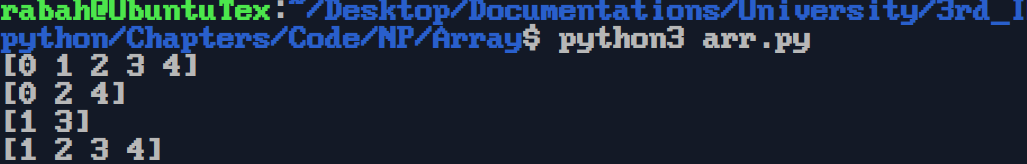
\includegraphics[width = 0.9\textwidth]{Chapters/ScreenShot/NP/Array/arOutput.png}
\end{center}

\vspace{1cm}



\textbf{\underline{LinSpace()}}\\[0.05cm]
\textbf{\underline{Syntax}}\\[0.1cm]
\lstinputlisting[style=pythonstyle]{Chapters/Code/NP/Array/syslin.py}

\vspace{0.5cm}

\textbf{\underline{Example}}\\[0.1cm]
\lstinputlisting[style=pythonstyle]{Chapters/Code/NP/Array/lin.py}

\vspace{0.25cm}
\begin{center}
    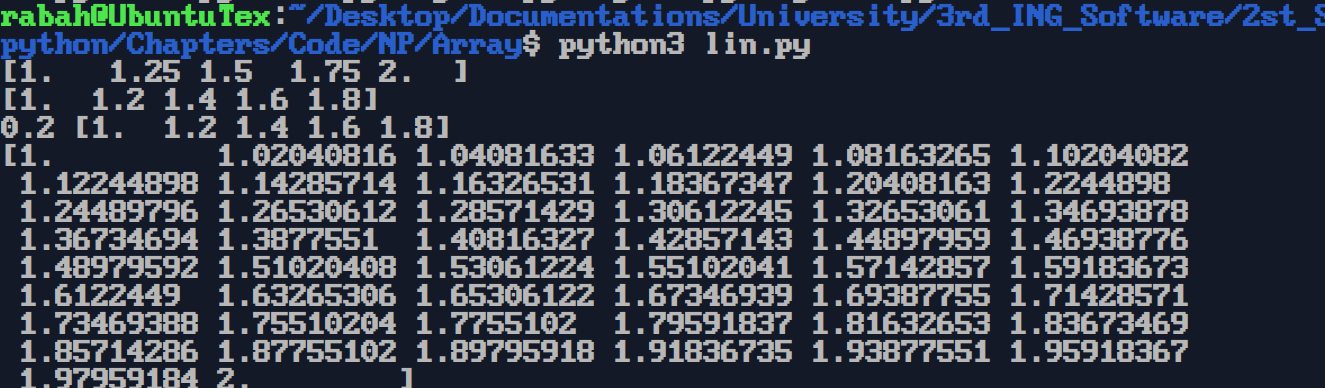
\includegraphics[width = 0.9\textwidth]{Chapters/ScreenShot/NP/Array/linOutput.png}
\end{center}

\vspace{1cm}

\subsection{Array Slicing}
\begin{prettyBox}{Slicing}{myblue}
\texttt{array[start=0 : stop=len(array) : step=1]}
\begin{itemize}
    \item \textbf{start} (default = 0): The index where slicing begins. If negative, it is interpreted as \texttt{len(array) + start}.
    \item \textbf{stop} (default = \texttt{len(array)}): The index where slicing ends (exclusive). If negative, it is interpreted as \texttt{len(array) + stop}.
    \item \textbf{step} (default = 1): Determines the stride between elements. Can be negative for reverse slicing.
\end{itemize}
\end{prettyBox}

\vspace{0.5cm}

\textbf{\underline{Example}}\\[0.1cm]
\lstinputlisting[style=pythonstyle]{Chapters/Code/NP/Array/slice.py}

\vspace{0.25cm}
\begin{center}
    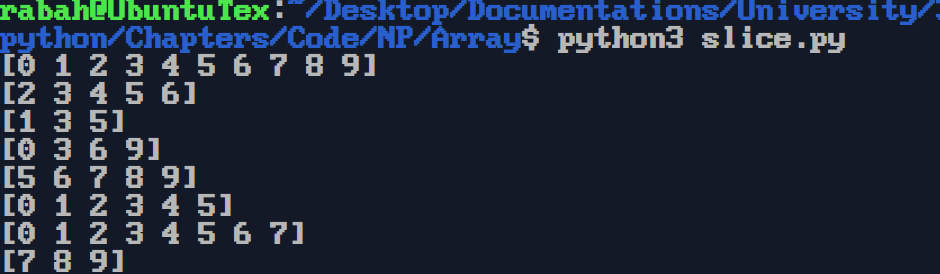
\includegraphics[width = 0.9\textwidth]{Chapters/ScreenShot/NP/Array/sliceOutput.png}
\end{center}

\newpage
\section{Mathematical Function}
\begin{prettyBox}{Function}{myblue}
\begin{itemize}
    \item \texttt{sin(x)} : \(\sin{(x)}\)  
    \item \texttt{cos(x)} : \(\cos{(x)}\)
    \item \texttt{tan(x)} : \(\tan{(x)}\)
    \item \texttt{exp(x)} : \(e^{x}\)
    \item \texttt{log(x)} : \(\ln{(x)}\) 
    \item \texttt{log10(x)} : \(\log_{10}{(x)}\)
    \item \texttt{log2(x)} : \(\log_{2}{(x)}\)
    \item \texttt{log(x) / log(b)} : \(\log_b{(x)}\)
\end{itemize}
\end{prettyBox}
